\documentclass[conference]{IEEEtran}
\usepackage{fancyhdr}
\usepackage{graphicx}
\usepackage{listings}
\usepackage{xcolor}
\usepackage{amsmath}
\usepackage{hyperref}
\usepackage{indentfirst}
\usepackage{titlesec}
\usepackage{subcaption}
\setlength{\marginparwidth}{2cm}
\usepackage{todonotes}
\hypersetup{
    breaklinks=true,
    urlcolor=blue,
    linkcolor=black,
    citecolor=black
}

\lstset{
    language=C,
    basicstyle=\ttfamily\small,
    stringstyle=\color{red},
    commentstyle=\color{blue}{},
    breaklines=true
}

\titlespacing*{\section}
{0pt}                      % left margin
{2ex plus 1ex minus .2ex}  % space before
{1ex plus .2ex}            % space after

\titlespacing*{\subsection}
{0pt}
{3ex plus 1ex minus .2ex}
{0.8ex plus .2ex}

\title{A Retrieval-Augmented Assistant for ASIC Design Debugging}
\author{
    \IEEEauthorblockN{Parker Schless (pis7)}
    \IEEEauthorblockA{ENMGT 5400: Applications of Artificial Intelligence for Engineering Managers \\
    Cornell University: School of Engineering Management}
}

\begin{document}
\maketitle

\section{Project Overview}
% Intro to asic design, problem in that there are so many very long generated documents
% Perfect opportunity for RAG
% What this project does: gather asic build outputs, performs intelligent chunking, embedding, and chromdb storing, then can query which embeds query, retrieves relevant documents, and passes question and context to LLM to get response
% Overview of results from eval

ASIC chip design is one of the most complex, detail-oriented processes in modern manufacturing. The latest chips contain billions of microscopic transistors, where any small error can lead to a total chip failure. As such, ASIC tool reports are incredibly verbose, often thousands of lines containing all the data dumped out from the tool runs. Moreover, many ASIC tools do not quit on failure, but rather just make a small note in the log and carry on. Chip designers must pore through these reports to discover any issues that arose during the run, which can take hours or even days at times.

With the rise of AI, chip designers are looking for new methodologies to ease this rather painful process. However, the length of these tool reports is not ideal even for such systems. If the user were simply to give the report to an LLM, the context window would quickly be consumed or even exceeded, leading to context rot and useless results.

\begin{figure}[ht]
    \centering
    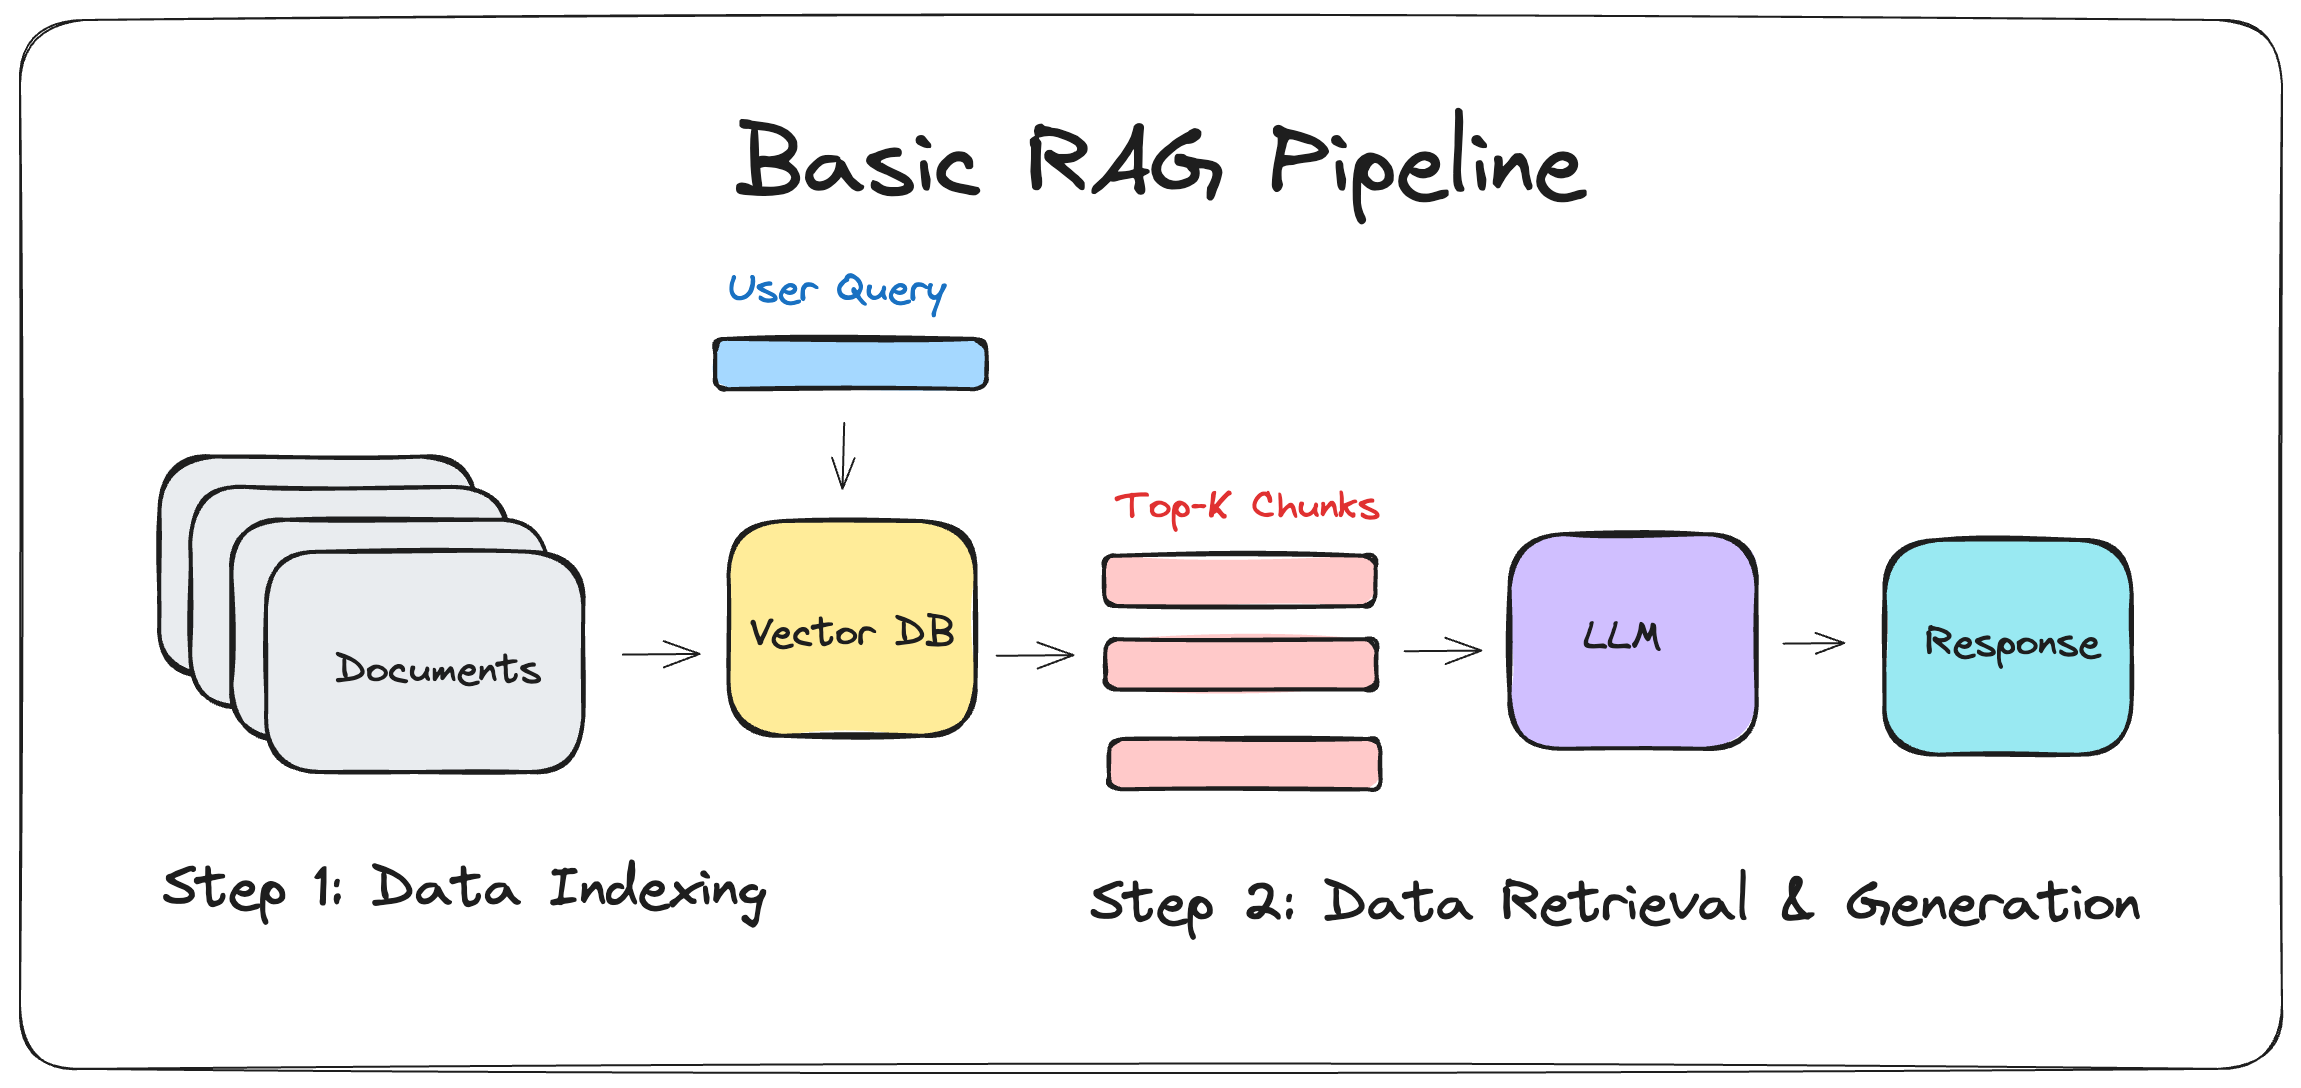
\includegraphics[width=\linewidth]{generic_rag.png}
    \caption{Generic RAG pipeline. Retrieved from \href{https://medium.com/@drjulija/what-is-retrieval-augmented-generation-rag-938e4f6e03d1}{Medium}.}
    \label{fig:generic_rag}
\end{figure}

Enter retrieval-augmented generation (RAG), a methodology for representing large documents in a series of lower-dimensional vectors to allow for more efficient context retrieval by LLMs \cite{lewis2020rag}. RAG works (Figure~\ref{fig:generic_rag}) by first splitting the source data, known as a corpus, into a series of "chunks." The way such chunks are made directly affects the quality of results -- using a naive fixed-chunking approach does not take into account document structure but is quite simple, whereas a structured-chunking approach more intelligently maps document sections into chunks at the cost of processing complexity. These chunks are then embedded into a vector form using an established embedding model and stored in a database format. For a given corpus, this process only needs to be performed once to generate the embedded vectors. 

When the user wishes to make a query on this database, the query is first embedded using the same method as for the chunks and sent to the database. The database will return the top $k$ chunks whose embedded vectors are closest in space to the query's embedded vector using cosine similarity. These chunks in text form are sent as context alongside the user query to the LLM to provide a more grounded answer without having to provide the LLM the entire corpus as context.

This project uses the concept of RAG in the context of ASIC chip design, where the corpus consists of the tool run outputs across a total of 475 files using 25MB of disk space. Using the custom-built pipeline, a series of queries are evaluated under different configurations using different chunking methodologies as well as additional techniques to improve QoR such as content-based filtering and chunk reranking. An analysis of the results and failure modes is then presented, where it is found that the best RAG configuration achieves a 3.7x improvement in answer correctness over the LLM alone, with structure-aware chunking providing the largest single gain. Error analysis reveals that retrieval and generation failures are evenly split, each accounting for 50\% of failures.

\section{Environment Setup}
% Zeppelin on FreePDK 45
% include pic of zeppelin on freepdk 45
% UV-based project, agile development and quick setup

While the intended use of RAG in this context is on real chip design projects that would be sent to the fab to be manufactured, NDA prevents the use of AI on restricted materials including the process development kits (PDKs). Luckily, there are a number of open-source PDKs available, such as NC State's \href{https://eda.ncsu.edu/freepdk/freepdk45/}{FreePDK45} 45nm process. As such, the first step of this project was getting a current chip tapeout project, the author's own Zeppelin/Blimp superscalar RISC-V processor, already implemented on TSMC180 set up with FreePDK45. This required a rework of the ASIC toolflow scripts and trial-and-error to get valid results (Figure~\ref{fig:zep_45_innovus}).

\begin{figure}[ht]
    \centering
    \includegraphics[width=\linewidth]{zep_45_innovus.png}
    \caption{Zeppelin superscalar processor implemented in FreePDK 45nm technology.}
    \label{fig:zep_45_innovus}
\end{figure}

Following the PDK setup, the services used for the RAG pipeline were chosen. For this project, quick bringup was the primary motivator, so the UV Python package manager was used to rapidly set up the Python environment, record package dependencies, and create script entry points. For the external API connections, OpenAI's \texttt{text-embedding-3-small} embedding model was used given its low price-point and simple Python API. For the vector database store, ChromaDB was chosen again due to its straightforward Python integration. Finally, Anthropic's Claude Sonnet model was chosen for the LLM given the author's familiarity with and existing subscription to the Claude ecosystem. The user's API keys for OpenAI and Anthropic are hidden from the pipeline in a \texttt{.env} file to provide security.

\section{System Architecture}
% Class-based approach, each script contains a main Executor class whose functions are executed in sequence
% corpus.py
% - contains collection rules (documents to obtain)
% - append a JSON segment for each relevant document found, contains source path, asic design variant, flow stage, asic tool, report type
% - dumps corpus JSON to file in build directory
% injest.py
% - calls a chunker, fixed or structured, returns list of chunks for each document
% - chunker.py - fixed chunker - creates fixed-sized chunks of each doucment (1500 characters per chunk with 200 character overlap)
% - chunker_structured - structured chunker - creates chunks with knowledge of sturcture of reports ahead of time, the key is the reports always have the same structure so easy to pre-define how we chunk, fixed-size fallback if cannot pre-define structure/not worth it to do so
% - initialize chromadb vector store
% - embed with OpenAI text-embedding-3-small with dimension 512 and batch size 32 chunks (tuned to produce good results with reasonable script runtime) and add to chromadb collection
% query.py
% - initialize Anthropic Claude Sonnet client
% - embed question with OpenAI embedding
% - can filter by asic design variant early on (field in data) to reduce available search space
% - return top_k (10) chunks
% - rerank if enabled - provide each of top_k chunks to claude and score based on relevance to question, goal is then to provide this to claude finally to give better QoR
% - format returned context nicely, give to claude as system prompt, and provide user question to get response

The RAG pipeline (Figure~\ref{fig:pipeline}) is built around a series of scripts using a class-based architecture for clean, understandable, and extensible code. For building the database of chunk vectors, the user first runs \texttt{corpus.py} to generate a JSON representation of all the source documents using a pre-defined set of document collection rules. Each entry in the JSON structure corresponds to a source document, with a field for the source path, ASIC design variant, ASIC flow stage, ASIC tool, report type, and the content of the document in whole. The additional fields are called metadata, and provide the subsequent chunking step with additional data to more intelligently split the document into chunks.

\begin{figure}[ht]
    \centering
    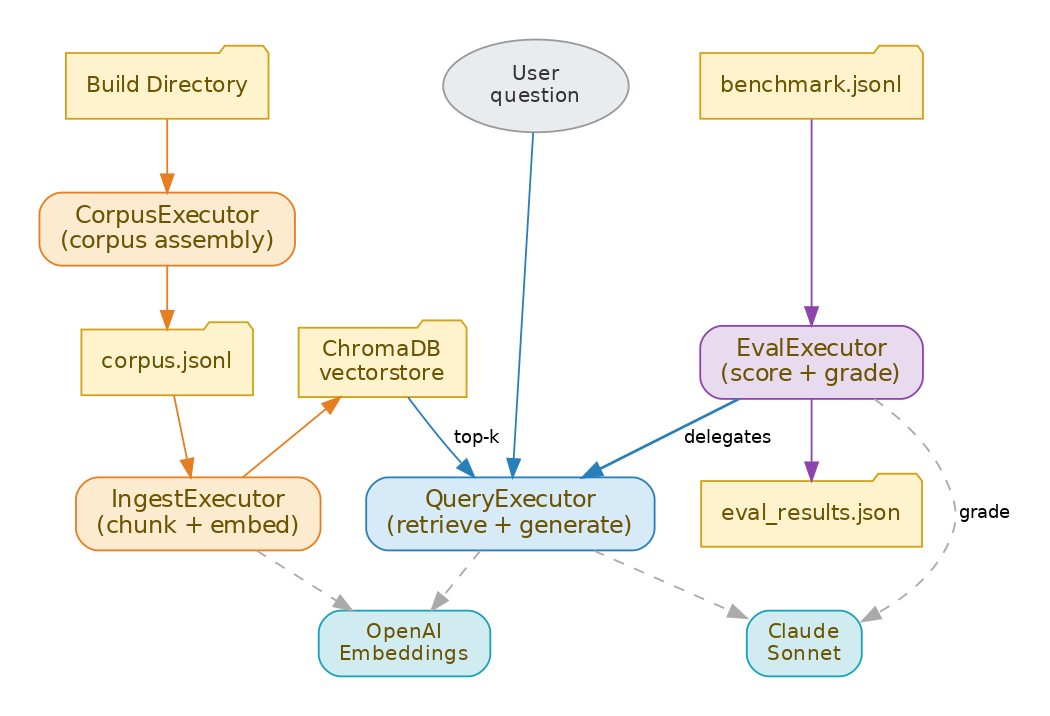
\includegraphics[width=\linewidth]{pipeline.png}
    \caption{ASIC design RAG pipeline implemented in Python with external API connections to OpenAI's \texttt{text-embedding-3-small} embedding model and Anthropic's Claude Sonnet LLM.}
    \label{fig:pipeline}
\end{figure}

After generating the JSON representation of the corpus, the data is then chunked. To evaluate the effectiveness of chunking, two such methods are used. One is the fixed-chunking approach where a source document is evenly split into chunks of 1500 characters with a 200 character overlap between each chunk to allow for better preservation of context at chunk boundaries. This chunk length was chosen based on the average length of relevant tool report sections. This approach is, obviously, not ideal for documents with a defined structure, where a more intelligent chunking scheme would better encapsulate relevant sections within the same chunk. As such, a structured-chunking scheme is also selectable which instead uses a predefined understanding of the contents of each document to create the chunks. The downside of this approach is that it only works on document structures that can be determined beforehand, which does in fact work well for ASIC toolflow results as reports will always have the same structure just with different data. As a fallback, however, the fixed-chunking scheme is used if the document type is unrecognizable via the associated metadata. 

Once chunking is complete, the resulting chunks are sent to the OpenAI embedding model to obtain a representative vector of dimension 512 and a batch size of 32. By default, the \texttt{text-embedding-3-small} model uses dimensionality of 1536, but this greatly increases the storage and cosine similarity calculation time. In the context of the standard use-case for RAG, a corpus of this size is actually on the small side, and so using a dimensionality of roughly 1/3 of the default has similar retrieval quality while improving on storage and calculation time efficiency. Once this vector is generated, it is stored in a ChromaDB database which can be accessed by the later query step.

Once the vector store is generated for a given corpus, the user need only run the query step for retrieving the relevant chunks and obtaining a response from the LLM. Since the user query must be compared to the vectorized chunks, it too needs to be embedded using the OpenAI model. Once this is complete, the ChromaDB database compares the query to the stored chunks using cosine similarity, which measures how closely aligned two vectors are in direction, returning the top chunks whose embeddings are most similar to the query. The database is configured to return the top 10 matching chunks which was experimentally found to provide enough context to the model to provide useful answers while not inducing context rot. Finally, the context chunks are provided to the Claude Sonnet LLM via the system prompt which also tells the model to act in the domain of ASIC chip design, as well as the question. A response is then generated through the API and returned to the user on the command line along with the source documents referenced for proper citation.

To further improve response quality, two additional features are implemented in the query step. The first is filtering the chunk selection by selected ASIC design. This is an optimization specific to this use case in that each corpus contains reports for multiple ASIC designs pushed through the flow. If the user includes an explicit mention to one of these designs in the prompt, the script will provide a filter to only look for reports for this specific design when fetching from the ChromaDB database. This filtering helps narrow down the search space to better improve relevance of retrieved documents. Additionally, reranking is also implemented where the returned chunks from the database are all given to the LLM to score based on relevance to the question. This acts as a sort of preprocessing step, where the resulting data is a ranked list of the returned chunks. This ranked list is then provided to the LLM once again along with the question to further narrow down the context when passing to the LLM. Both of these options are able to be switched on and off, as is done in the evaluation section to test their effectiveness.

\section{Evaluation and Error Analysis}
% corpus: 475 documents, 25MB, RTL source, sdc onstraints, timing reports, area reports, power reports, drc/lvs logs, flow summaries, build configs
% 30 questions asked to system similar to those I asked during development of Zeppelin, split across four categories of simple lookup, cross-document, cross-variant, and general reasoning
% metrics included retieval recall - how well did the top-k retrieved chunks include the expected source documents, and answer quality based on correctness and completion
% tested the 30 questions across 6 strategies varying chunking structure, variant filtering, and reranking
% failure analysis with 4 categories - retrieval hit/miss with good/bad answer

\subsection{Metrics}

To evaluate the effectiveness of the RAG pipeline, a benchmark of 30 questions with expected sample responses and retrieval source documents are tested on the pipeline. Each benchmark is then provided to the LLM in a separate instance to grade the generated responses based on retrieval quality (do the retrieved chunks contain the expected source documents), answer correctness (does the answer contain the key facts), and answer completeness (does the answer address all parts of the question) on a scale from 0 to 3. The 30 questions are split into four categories as shown in Table~\ref{tab:benchmark_categories}.

\begin{table}[h]
\centering
\caption{Benchmark question categories}
\begin{tabular}{lrl}
\hline
\textbf{Category} & \textbf{Count} & \textbf{Description} \\
\hline
Simple-lookup    & 12 & Single-fact retrieval \\
Cross-document   &  5 & Comparing metrics across flow stages \\
Cross-variant    &  7 & Comparing metrics across design variants \\
Reasoning        &  6 & Architectural understanding and explanation \\
\hline
\end{tabular}
\label{tab:benchmark_categories}
\end{table}

Additionally, five configurations of the RAG pipeline are tested as shown in Table~\ref{tab:rag_configs}.

\begin{table}[h]
\centering
\caption{RAG configurations tested}
\begin{tabular}{lp{5cm}}
\hline
\textbf{Configuration} & \textbf{Description} \\
\hline
No context (LLM only)       & Claude answers with no retrieved context (baseline) \\
Fixed chunking              & 1500-char sliding window, 200-char overlap \\
Structured chunking         & Structure-aware chunking (section headers, benchmark blocks, timing paths) with metadata prefixes; splits summary log header into semantic sub-groups \\
Struct + variant filter     & Auto-detects variant name in question and filters results to that variant's chunks \\
Struct + filter + rerank    & Additionally re-ranks retrieved chunks using Claude as a relevance judge \\
\hline
\end{tabular}
\label{tab:rag_configs}
\end{table}

\subsection{Evaluation}

The results of the benchmark are tabulated by strategy in Table~\ref{tab:benchmark_results_strat} and by benchmark category in Table~\ref{tab:benchmark_results_categ}. 

\begin{table}[h]
\centering
\caption{Evaluation results across RAG configurations}
\begin{tabular}{lccc}
\hline
\textbf{Strategy} & \textbf{Recall} & \textbf{Correct. (/3)} & \textbf{Complete. (/3)} \\
\hline
No context (LLM only)       & n/a  & 0.57 & 0.53 \\
Fixed chunking              & 0.38 & 1.40 & 1.80 \\
Structured chunking         & 0.48 & 2.13 & 2.37 \\
Struct + variant filter     & 0.63 & 2.07 & 2.23 \\
Struct + filter + rerank    & 0.63 & 2.13 & 2.30 \\
\hline
\end{tabular}
\label{tab:benchmark_results_strat}
\end{table}

\begin{table}[h]
\centering
\caption{Correctness results by category: best RAG config vs.\ no context}
\begin{tabular}{lccc}
\hline
\textbf{Category} & \textbf{No Context} & \textbf{Best RAG} & \textbf{Improvement} \\
\hline
Simple-lookup    & 0.25/3 & 2.83/3 & 11x \\
Cross-document   & 0.00/3 & 1.60/3 & from 0 \\
Cross-variant    & 0.00/3 & 1.43/3 & from 0 \\
Reasoning        & 2.33/3 & 2.00/3 & $-14\%$ \\
\hline
\end{tabular}
\label{tab:benchmark_results_categ}
\end{table}

It is seen that the structured chunking with filtering and reranking configuration achieves the highest answer correctness at 2.13/3, a 3.7x improvement compared to using no RAG at all. Adding variant filtering and reranking improves retrieval recall from 0.48 to 0.63 but does not further improve correctness beyond structured chunking alone. Across the simple-lookup category, RAG provides an 11x improvement. When not using RAG, the LLM is not able to answer project-specific factual questions at all with correctness scores of 0 for both cross-document and cross-variant benchmarks, and near 0 for simple-lookup queries.

Another finding is that structured chunking provided a correctness improvement of 1.52x over fixed chunking. This reveals that chunking based on known document semantics which in this case were at section headers, benchmark blocks, and metric groups produced far better embeddings which more closely aligned with the targeted questions. Variant filtering with structured chunking also provided a retrieval recall improvement of 1.31x over structured chunking only (0.48 to 0.63). While not as significant an improvement to answer correctness as structured chunking vs fixed chunking, this still shows that metadata-aware retrieval does in fact help to narrow down the search space and thus improve quality of results. Re-ranking seemed to slightly improve the quality of the answers in terms of both correctness (1.03x) and completeness (1.03x) but not the recall score. This makes sense given re-ranking reorders the retrieved chunks based on relevance but doesn't change which chunks are retrieved.

Finally, the reasoning category received a better correctness score when not using RAG as opposed to when using RAG (a 14\% regression). Much of this category is based around generic knowledge of the task at hand, which in this case is ASIC chip design. It turns out that Claude has a decent understanding of the basics as discovered through the author's testing, but when supplying the model with project-specific knowledge, it often gets confused since this context is not needed in these cases, and answer quality degrades as a result. An improvement to this system may be including a retrieval confidence threshold which skips appending the retrieved context if the threshold is below a user-tuned value.

\subsection{Error Analysis}

After performing evaluation of the benchmarks, the failure cases are then examined to determine improvements that can be made to the system. The failure cases are documented in Table~\ref{tab:failure_classification} which classifies such failures into four categories as combinations of whether the retrieval was good or bad and whether the answer was good or bad.

\begin{table}[h]
\centering
\caption{Failure classification (best RAG config, 30 questions)}
\begin{tabular}{lrl}
\hline
\textbf{Category} & \textbf{Count} & \textbf{Description} \\
\hline
Retrieval hit + good answer  & 16/30 & System working as intended \\
Retrieval miss + good answer &  6/30 & LLM compensated \\
Retrieval miss + bad answer  &  4/30 & Retrieval failure \\
Retrieval hit + bad answer   &  4/30 & Generation failure \\
\hline
\end{tabular}
\label{tab:failure_classification}
\end{table}

Overall, the LLM succeeded (good answer regardless of retrieval status) in 22/30 cases, which is reasonable given the simplicity of this RAG pipeline. In general, 50\% of the failures were a result of retrieval misses leading to bad answers, while 50\% of the failures were a result of a good retrieval but the LLM producing an invalid response. Based on this, retrieval and generation failures are evenly split, and both represent significant avenues for improvement.

\section{Conclusion}
% limitations
% high level conclusions from eval and error analysis

Overall, the RAG pipeline built for this project improved the answer quality generated by the LLM for 70\% of the queries in the benchmark suite, while hurting the answer quality for 10\% of the questions, all of which involved general reasoning. The remaining 20\% of the benchmark suite produced answers that were neither better nor worse with or without RAG according to the grading metric. Of the failure cases, retrieval and generation failures were evenly split at 50\% each.

Known limitations of the constructed pipeline include, for one, a limited corpus that only contains design artifacts (reports, logs, source RTL) and no EDA tool documentation. While the author had desired to include this documentation as part of the corpus, non-redistribution agreements prevented this, and surely resulted in a loss of answer quality. Additionally, the chosen embedding model, like most embedding models, was trained primarily on web text, and not on ASIC-specific terminology such as "synth\_setup\_slack" or "pnr\_density." Fine-tuning such an embedding model would likely yield better results. Finally, improvements could be made to the evaluation methodology, particularly by including more benchmark questions to provide more statistical confidence in the results, as well as reducing grading bias given that Claude is essentially grading output generated by itself.

In the end, a RAG pipeline with a 70\% evaluation suite improvement built with open-source tools and implemented in a concise 1300-line codebase is a notable achievement, and the suggested avenues for further optimization would surely result in even better performance if implemented.

\section{AI Attribution}
Claude Code was used heavily for this project. It was used in the beginning phases to evaluate embedding and LLM APIs in terms of their cost, implementation complexity, and availability for use in this project. After settling on the APIs to use, Claude Code was used to turn the author's high-level architectural specification into real code, with specific tweaks and refactors being incrementally performed during debugging and optimization sessions. Claude Code also built the benchmark script and helped evaluate and tabulate the results. Finally, Claude Code was used to help proofread this report for grammar and spelling mistakes, as well as for clarity and technical improvements.

\bibliographystyle{IEEEtran}
\bibliography{references}

\end{document}